\chapter{Laboratorium 5}
\section{Wstęp teoretyczny}
\subsection{Format BMP}
Format BMP został stworzony do grafiki bitmapowej\cite{bmp}. W strukturę tego formatu wchodzi nagłówek oraz tabela pikseli. W nagłówku zapisane są wszelkie informacje na temat charakterystyki bitmapy z których najważniejsze to: wysokość, szerokość, oraz liczba bitów na piksel. Jest to istotne, gdyż te wartości wpływają na budowę tabeli pikseli [Rysunek {\ref{fig:BMP}]. Istotna jest także jej budowa, gdyż tabela pikseli jest zapisana od dołu do góry, od lewej do prawej. Oznacza to, iż dolny lewy róg jest jej początkiem, a prawy góry róg - końcem. Ważny jest też \textit{padding}, gdyż w strukturze ilość bajtów w każdym wierszu musi być potęgą liczby 4.

\begin{figure}[H]
\centering
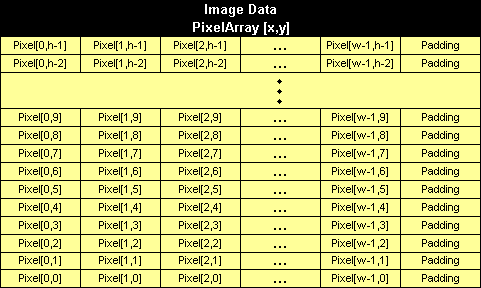
\includegraphics[height=6cm]{images/bmp.png}
\caption{tabela pikseli}
\label{fig:BMP}
\end{figure}

\subsection{Architektura MMX}
Jest ona wykorzystywana głównie przetwarzania dużych ilości danych gdzie wykorzystywany jest jeden algorytm. Najważniejszymi cechami tejże architektury są\cite{userguide}:
\begin{itemize}
\item 8 rejestrów 64 bitowych wykorzystujących rejestry FPU (MM0 - MM7).
\item typ danych "packed". Jego działanie polega na traktowaniu rejestru 64 bitowego jako wektora pewnej liczby komórek o tej samej wielkości.
\item format instrukcji. Instrukcje dla MMX budowane są w kolejności: \textbf{P}, skrót rozkazu/instrukcja (np. \textbf{ADD}), litery \textbf{S} dla wartości ze znakiem bądź \textbf{U} dla wartości bez znaku, \textbf{S} jeśli operacja jest wykonywana z nasyceniem, litery \textbf{L} lub \textbf{H} jeśli operacja wykonywana jest na mniej lub bardziej znaczących bitach oraz \textbf{B}, \textbf{W}, \textbf{D}, \textbf{Q} które odpowiadają za rozmiar komórki wektora. Przykładowa instrukcja MMX: \textbf{PADDUSB} (równoległe dodawanie, bez znaku z saturacją, bajtów).
\end{itemize}
\section{Zakres prac}
Zadaniem było stworzenie programu w C który wczytywał by plik graficzny (bmp, jpg) i wprowadzałby na nim filtry (odbicia poziome, pionowe oraz po przekątnej, saturacja, negatyw). Następnie należało wybrany filtr napisać w ASM, i porównać czas działania funkcji w C i ASM.
\section{Rozwiązanie}
Do stworzenia funkcji w C można było wykorzystać gotowy schemat ze strony \textit{Zakładu Architektury Komputerów}\cite{zak} który potrafił wczytać oraz zapisać pliki graficzne. Przed przystąpieniem do tworzenia filtrów zostały do kodu programu dodane dwie zmienne (\ref{l:zmienne}): \textit{rowSize} odpowiedzialne za długość wiersza w tablicy pikseli oraz \textit{padding} będące wartością paddingu w aktualnie wczytanym pliku. 

\begin{lstlisting}[language=C, frame=single, caption=Dodatkowe zmienne , label=l:zmienne, basicstyle=\small]  
int rowSize = 
	(( image->format->BitsPerPixel * image->w + 31) / 32) * 4;
int padding = 
	4 - ( (image->w * image->format->BytesPerPixel) % 4);
\end{lstlisting}

\subsection{Operacje na tabeli pikseli}
Przestawianie pikseli w tablicy pikseli należy do trudniejszych zadań. Należy pamiętać o kolejności wierszy w pliku, nie można zapomnieć o występowaniu paddingu co utrudnia operacje przeprowadzane za pomocą prostych pętli for, poza tym działamy na macierzy jednowymiarowej interpretowanej później jako macierz dwuwymiarowa. Dla przykładu kod w \ref{l:vertical} przedstawia prostszą funkcję zmieniającą kolejność pikseli. W tym przypadku nie potrzebna nam była wartość \textit{paddingu}. Jest to prosta suma pętli która zamienia piksele miejscami. W poziomie zakres jest od 0 do wartości \textit{rowSize}. Dużo trudniejsze było napisanie funkcji która odbijała by obraz po przekątnej (\ref{l:diagonal}). Przydała się tam wartość \textit{paddingu} dzięki której można było w szybki sposób ograniczać działanie na tablicy.
Najistotniejsze jednakże jest to, aby przenosić wartości pełnych pikseli, a nie wyłącznie kolejne bajty, gdyż wtedy możemy zakłócić kolory poszczególnych pikseli.
\newpage
\begin{lstlisting}[language=C, frame=single, caption=Funkcja odbijająca obraz w pionie , label=l:vertical, basicstyle=\small]  
void verticalFilter(unsigned char * buf, int width,
		int height,int size,char bpp, int rowSize)
{
  int i, j, k;
  char temp;
    for(i=0; i < (height/2) ; i++)
    {
      for(j=0; j < (width*bpp); j++)
      {
        temp = buf[(i *rowSize) +j];
        buf[ (i *rowSize) +j] = buf[ ((height-i-1) *rowSize) +j ];
        buf[ ((height-i-1) *rowSize) +j ] = temp;
      }
    }
}
\end{lstlisting}

\begin{lstlisting}[language=C, frame=single, caption=Funkcja odbijająca obraz po przekątnej , label=l:diagonal, basicstyle=\small]  
void diagonalFilter(unsigned char * buf, int width,
	int height,int size,char bpp, int RowSize, int Padding)
{
  int i, j, k;
  char temp;
  for(i=0; i < height/2; i++)
  {
    for(j=0; j < (width); j++)
    {
      for(k=0; k<bpp; k++)
      {
        temp = buf[ ( i *(RowSize) ) + ( j *bpp ) +k ];
        
        buf[ ( i * RowSize) ) +( j *bpp ) +k ] = buf[ ( (height-
        i) * (RowSize) - Padding ) - ( j * bpp ) + k ];
        
        buf[ ( (height-i) *(RowSize) -Padding ) - 
        ( j *bpp ) +k ] = temp;
      }
    }
  }
}
\end{lstlisting}

\subsection{Operacje na wartościach pikseli}
Dużo łatwiejsze jest przeprowadzanie tej samej operacji na wartościach pikseli. W przypadku negatywu (\ref{l:negat}) sprawa wygląda dość prosto. Wystarczy zanegować wartości każdego bajta, i w ten sposób otrzymujemy obraz w negatywie. Operacje na poszczególnych pikselach są o tyle łatwiejsze, że uruchamiamy odpowiednio przygotowany algorytm na każdym kolejnym wektorze bajtów, bez potrzeby zastanawiania się jak są one rozmieszczone w tabeli pikseli.
\begin{lstlisting}[language=C, frame=single, caption=Funkcja odbijająca obraz w pionie , label=l:negat, basicstyle=\small]  
void negativeFilter(unsigned char * buf, int width,
		int height,int size,char bpp, int RowSize)
{
  int i, j, k;
  char temp;
  for(i=0; i < height ; i++)
  {
    for(j=0; j < (width*bpp); j++)
    {
      buf[ (i*RowSize) + j] = (~buf[ (i*RowSize) + j]);
    }
  }
}
\end{lstlisting}

\section{Wnioski}
Laboratorium nauczyło mnie jak zbudowane są pliki graficzne. Pozwoliło to także zrozumieć sposób w jaki działają programy graficzne, jak działają filtry czy rysowanie. Zapewne po utworzeniu funkcji która konwertowałaby wektor jednowymiarowy w dwuwymiarowy, praca nad filtrami była by dużo prostsza a i kod byłby dużo prostszy w czytaniu. Niestety ze względu na trudność w początkowym zrozumieniu pracy nad tablicą trójwymiarową zapisaną jako wektor jednowymiarowy nie udało się podczas zajęć laboratoryjnych stworzyć kodu w ASM a także porównać czas działania. Mogę wyłącznie przewidywać, że czas działania będzie przynajmniej kilka razy większy ze względu na możliwość działania na kilku wartościach jednocześnie, co podobne w działaniu jest do pracy na wątkach.